% !TeX root = ../main.tex

\chapter{算法设计}

我们设计了两种算法来对问题 (\ref{problem}) 进行求解:

\begin{enumerate}
  \item \textbf{随机化中值查找算法} \cite{10.1016/j.patcog.2017.02.006}:该算法的核心思想是通过将断点分割为 $L$ 集合和 $G$ 集合,其中 $L$ 集合中储存小于当前断点的断点下标,$G$ 集合中储存大于当前断点的断点下标。在分割完成后,通过判断 $g(x)$ 的符号来确定如何求解原问题 (\ref{problem})。
  \item \textbf{排序后二分查找算法} \cite{10.5555/1577069.1755859}:该算法的核心思想是通过将断点进行从小到大的排序,而后使用二分法查找最终解。
\end{enumerate}

随机化中值查找算法的伪代码如算法 (\ref{Algorithm:RMFA}) 所示:

\medskip

\begin{algorithm}[H]
  \SetStartEndCondition{ }{}{}
  \SetKwIF{If}{ElseIf}{Else}{if}{:}{elif}{else:}{}
  \SetKwFor{While}{while}{:}{fintq}
  \AlgoDontDisplayBlockMarkers\SetAlgoNoEnd\SetAlgoNoLine
  \KwData{$a,b,c,d,breakpoints$}
  \KwResult{$x^*(x^*\in\mathbb{R}\text{ and }0\in g(x^*))$}

  $x\longleftarrow breakpoints,k\longleftarrow 0,x_k\longleftarrow x[k],g_k\longleftarrow g(x_k)$\;
  $U\longleftarrow \{0,1,\dots,[x]\}$\;
  \While{$U\neq \emptyset$}{
    $k\longleftarrow choice(U),x_k\longleftarrow x[k]$\;
    $L\longleftarrow\{i\mid x_i<x_k, i\in U\},G\longleftarrow\{i\mid x_i\geq x_k, i\in U\}$\;
    $g_k\longleftarrow g(x_k)$\;
    \eIf{$g_k<0$}{
      $g_k\longleftarrow g_k+|b_k|$\;
      \eIf{$g_k\geq 0$}{
        break\;
      }{
        $U\longleftarrow G\setminus k$\;
      }
    }{
      $U\longleftarrow L$\;
    }
    \If{$U=\emptyset$}{
      $x_k\longleftarrow x_k-g_k/a$\;
      break\;
    }
  }
  \Return{$x_k$}\;
  \caption{随机化中值查找算法}\label{Algorithm:RMFA}
\end{algorithm}

排序后二分查找算法的伪代码如算法 (\ref{Algorithm:DFAS}) 所示:

\medskip

\begin{algorithm}[H]
  \SetStartEndCondition{ }{}{}
  \SetKwIF{If}{ElseIf}{Else}{if}{:}{elif}{else:}{}
  \SetKwFor{While}{while}{:}{fintq}
  \AlgoDontDisplayBlockMarkers\SetAlgoNoEnd\SetAlgoNoLine
  \KwData{$a,b,c,d,breakpoints$}
  \KwResult{$x^*(x^*\in\mathbb{R}\text{ and }0\in g(x^*))$}

  $x\longleftarrow sorted(breakpoints),start\longleftarrow 0,end\longleftarrow len(x)-1$\;
  \While{$True$}{
    $mid\longleftarrow\lfloor\frac{start+end}{2}\rfloor$\;
    \eIf{$g(x[start])\cdot g(x[end]<0)$}{$end\longleftarrow mid$\;}{$start\longleftarrow mid$\;}
    \If{$end-start=1$}{
      $root\longleftarrow x[end]-\frac{g(x[end])}{a}$\;
      \eIf{$g(root)=0$}{
        \Return{$root$}\;
      }{
        \Return{$x[start]$}\;
      }
    }
  }
  \caption{排序后二分查找算法}\label{Algorithm:DFAS}
\end{algorithm}

可以证明,算法 (\ref{Algorithm:RMFA}) 的时间复杂度是 $O(m)$,其中 $m$ 是断点的数量 \cite{10.1016/j.patcog.2017.02.006},而算法 (\ref{Algorithm:DFAS}) 的时间复杂度取决于时间复杂度为 $O(m\log{m})$ 的排序算法。

对于给定数据 $a=1.5,d=1,b=[1;1.2;−0.9],c=[0.1;−1.4;−1.2]$,使用上述两个算法求解结果如图 (\ref{Answer}) 所示(紫色点即为求解结果):

\begin{figure}[htb]
  \centering
  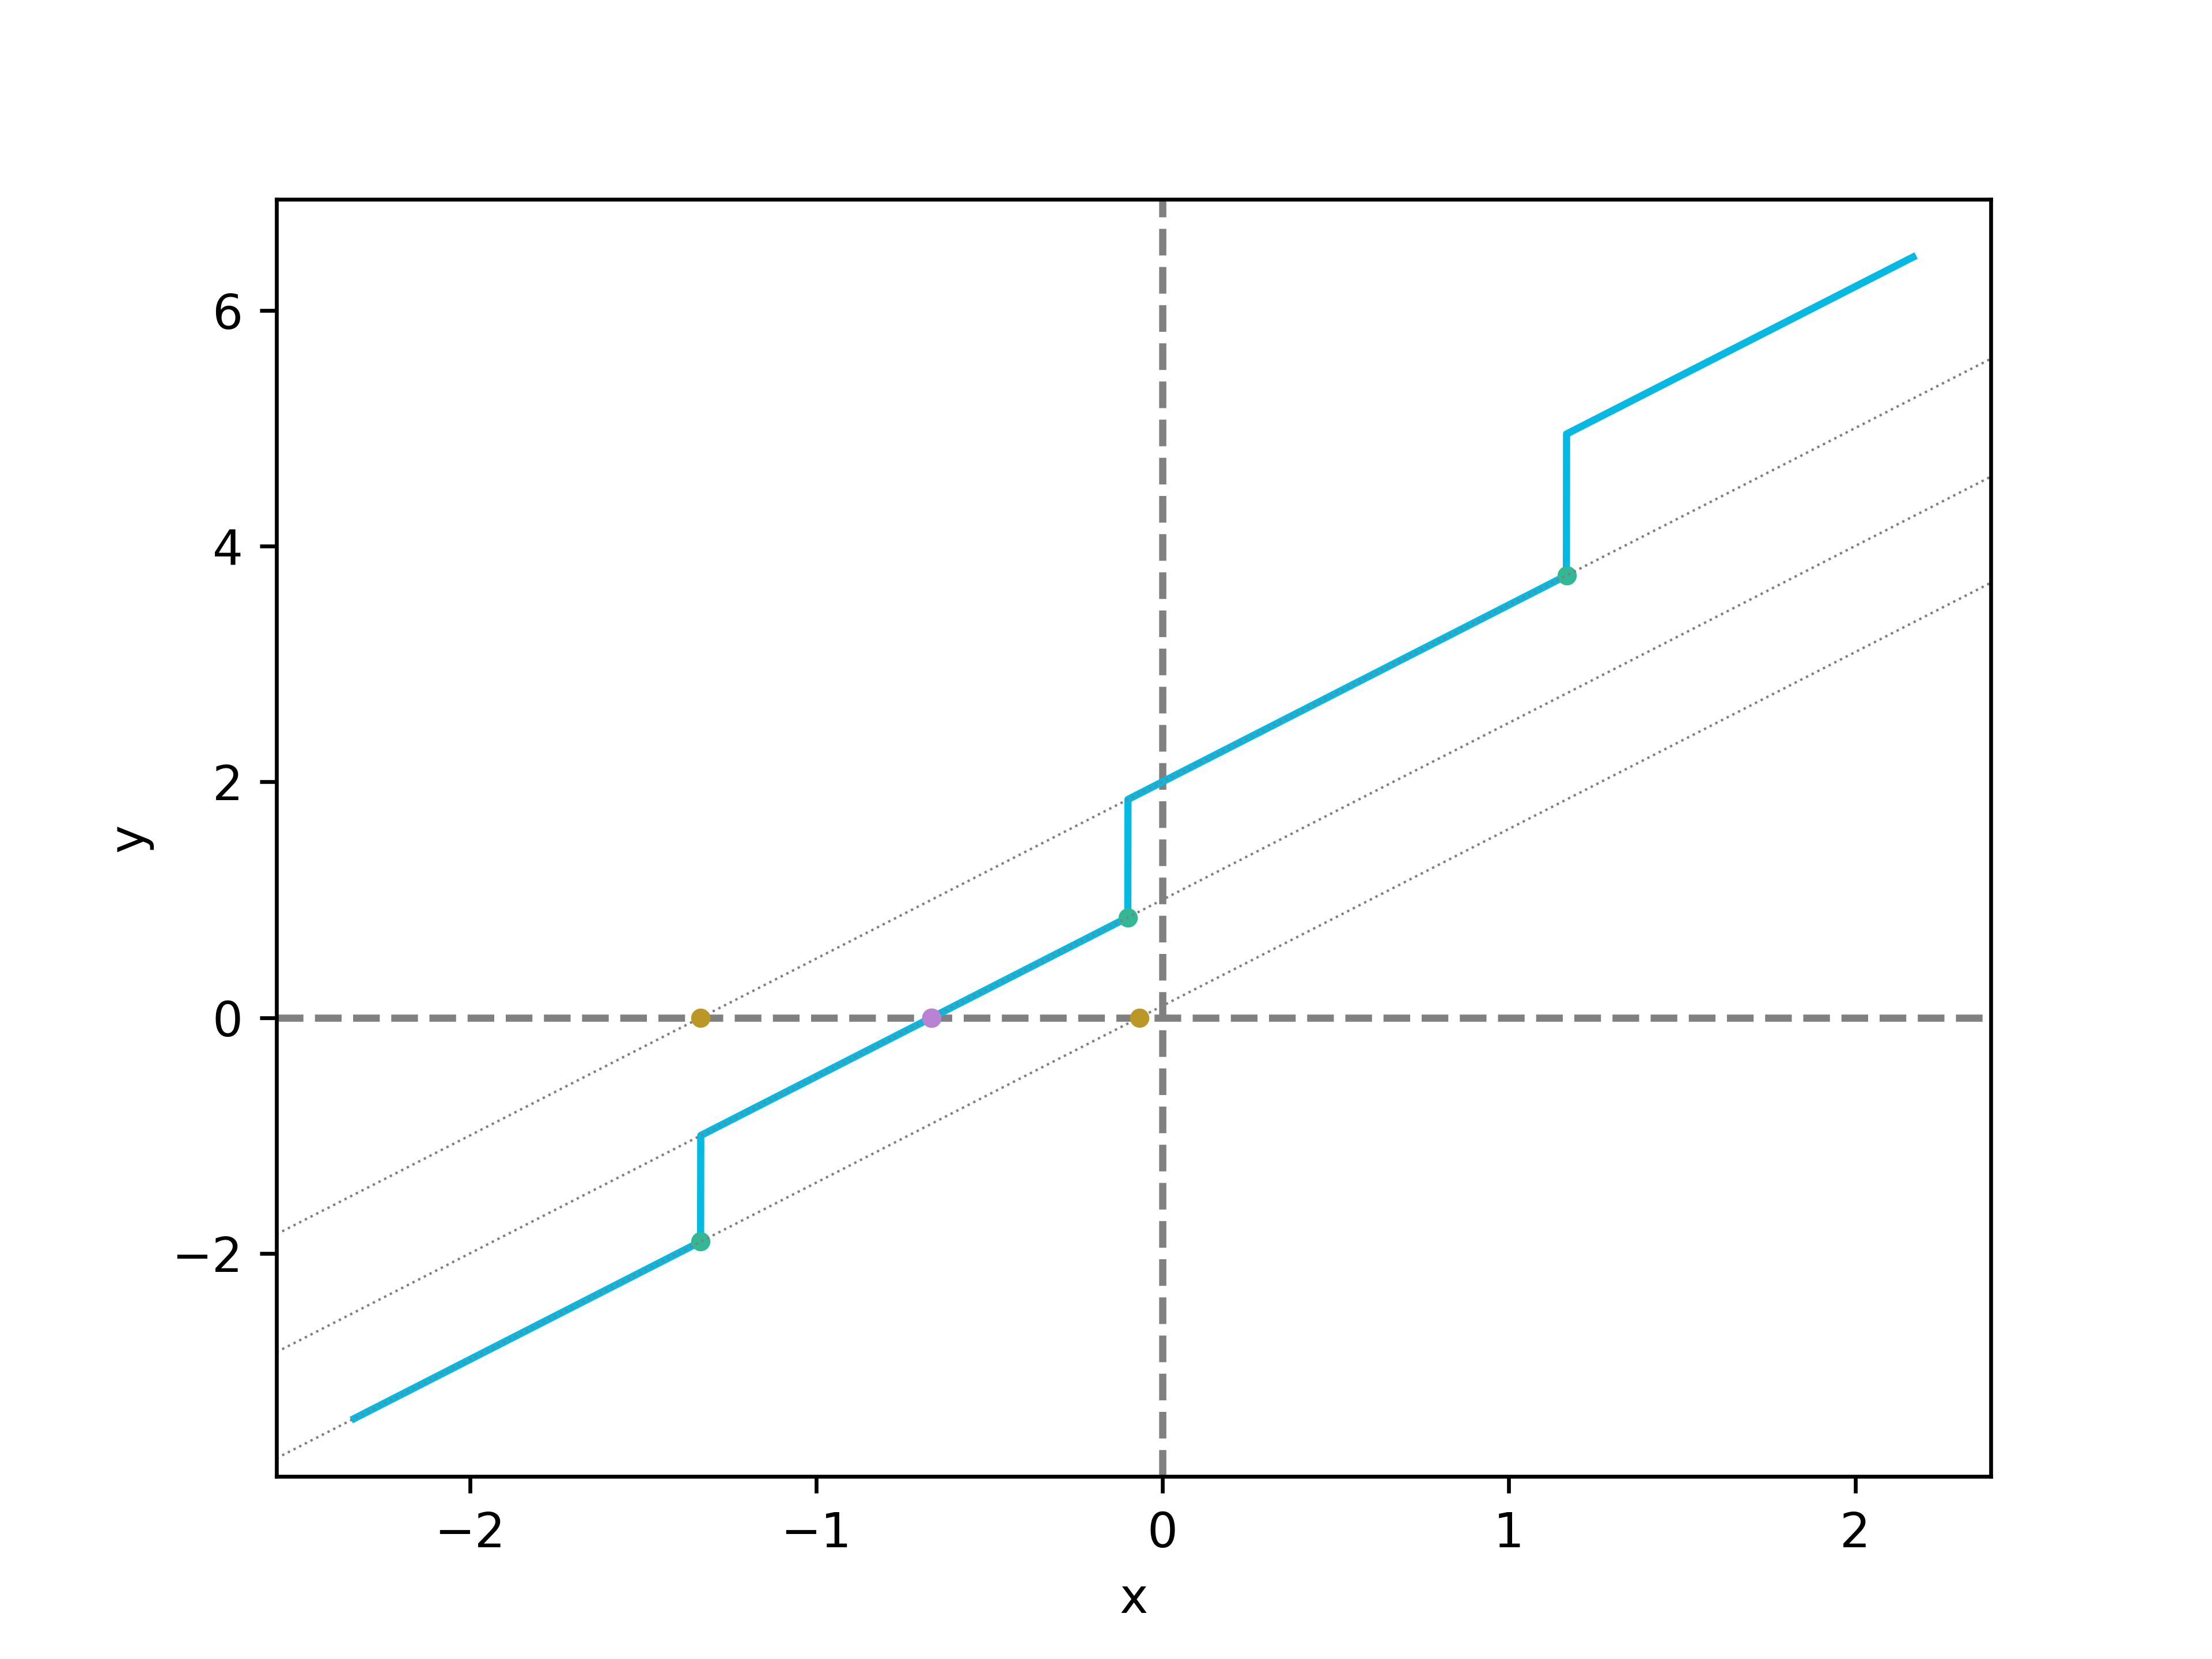
\includegraphics[width=0.5\textwidth]{figures/Answer.png}
  \caption{求解结果}
  \label{Answer}
\end{figure}

如图 (\ref{Answer}) 所示,两个算法的求解结果重合并且均在 $x$ 轴上,即所求解结果是正确的。